\documentclass{article}
\usepackage{pgf}
\usepackage{tikz}
\usetikzlibrary{arrows,automata}
\usepackage[latin1]{inputenc}
\usepackage{listings}
\lstdefinestyle{customc}{
  belowcaptionskip=1\baselineskip,
  breaklines=true,
  frame=L,
  xleftmargin=\parindent,
  language=C,
  showstringspaces=false,
  basicstyle=\footnotesize\ttfamily,
  keywordstyle=\bfseries\color{green!40!black},
  commentstyle=\itshape\color{purple!40!black},
  identifierstyle=\color{blue},
  stringstyle=\color{orange},
}
\lstset{escapechar=@,style=customc}
\begin{document}
\begin{figure}
\center
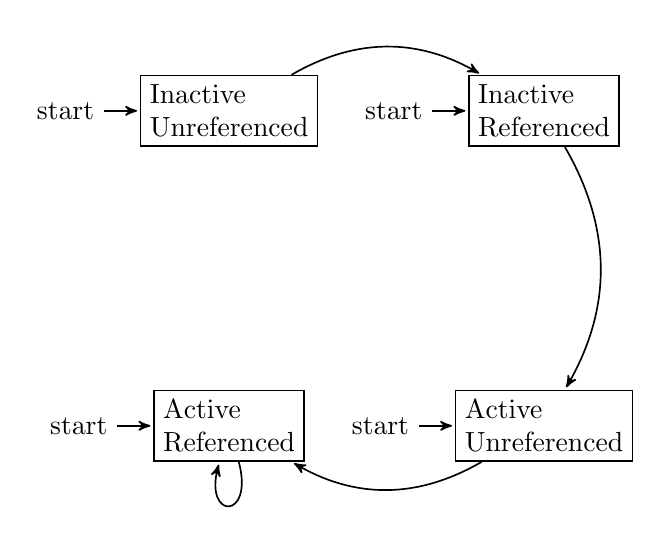
\begin{tikzpicture}[->,>=stealth',shorten >=1pt,auto,node distance=4cm,
                    semithick]

  \tikzstyle{every state}=[rectangle,draw,align=left]

  \node[initial,state] (IU)               {Inactive \\ Unreferenced};
  \node[initial,state] (IR) [right of=IU] {Inactive \\ Referenced};
  \node[initial,state] (AU) [below of=IR] {Active \\ Unreferenced};
  \node[initial,state] (AR) [below of=IU] {Active \\ Referenced};

  \path (IU) edge [bend  left] node {} (IR)
        (IR) edge [bend  left] node {} (AU)
        (AU) edge [bend  left] node {} (AR)
        (AR) edge [loop below] node {} (AR);
\end{tikzpicture}
\caption{Classic}
\end{figure}
\begin{figure}
\center
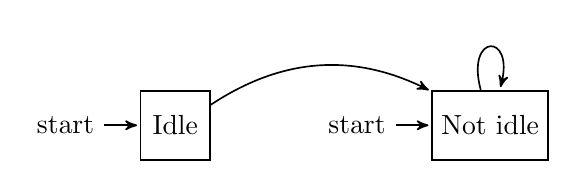
\begin{tikzpicture}[->,>=stealth',shorten >=1pt,auto,node distance=4cm,
                    semithick]

  \tikzstyle{every state}=[rectangle,draw,align=left]

  \node[initial,state] (IL)               {Idle};
  \node[initial,state] (NI) [right of=IL] {Not idle};

  \path (IL) edge [bend  left] node {} (NI)
        (NI) edge [loop above] node {} (NI);
\end{tikzpicture}
\caption{Idle page tracking}
\end{figure}
\lstinputlisting[caption=mark\_page\_accessed, style=customc]{src/mark_page_accessed.c}
\end{document}
